\documentclass[Rapport]{subfiles}
\begin{document}

\section{Framtida arbete}

En avgränsning för vårt projekt var att jobba inom ramen för en interpreter. 
Detta av flera anledningar, men främst för att det är lättare att göra prototyper för 
olika regler för optimise. Nu när vi har tagit fram fungerande optimeringssemtantik 
är nästa steg att implementera vårt språk i en kompilator.
Med callstacken istället för substitutionsfunktionen tror vi att implementationen
i en kompilator skulle vara mer realiserbar.


Vårt core språk liknar det som både YHC och GHC arbetar med i sina mellansteg.
Det hade varit ytterst intressant att utöka vårt språk så att vi skulle kunna 
vara backend till något större kompilator, eller runtimesystem?
Vi har alltid haft detta i åtanke och det är delvis därför vi ej har någon 
typechecker.


\NOTE{
Info bild som visar en pipe line för vart vår kompilator finns i kedjan.

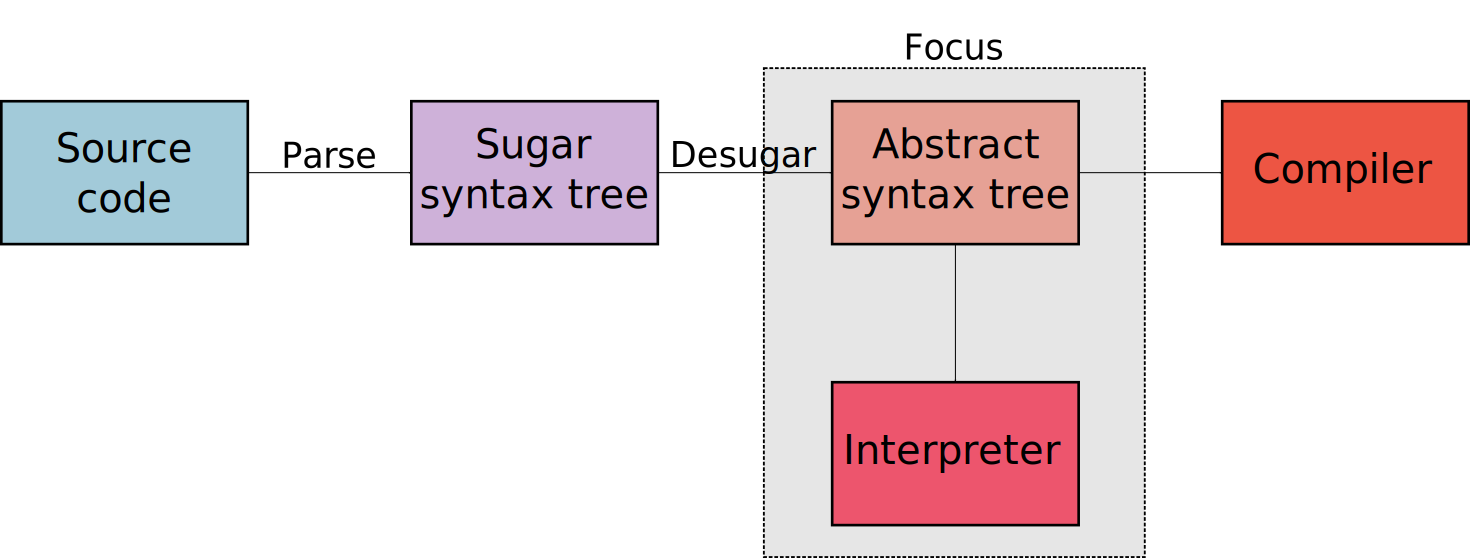
\includegraphics[scale=0.22]{img/pipeline} 
}


En typechecker och stöd för t ex algebric datatypes i ett frontend hade också
varit trevligt då det är väldigt lätt att skriva fel i testprogramen. 


Något annat som föll lite utanför ramen för vårt arbete är att bevisa
korrektheten hos optimisefunktionen, för att se att en optimerad funktion
gör samma sak som dess ooptimerade motsvarighet. Vi har endast använt oss av en testsvit
och andra exempelprogram för att testa optimise. Ett steg för att förvissa sig
om korrektheten skulle vara att göra QuickCheck-egenskaper och generatorer för att se
att en optimerad funktion gör samma sak som en ooptimerad. En annat sätt för att vara säker på att den
gör vad som förväntas vara att formalisera reglerna och bevisa
att de är korrekta, exempelvis med hjälp av en bevisassistent såsom Agda.


\subsection{Utveckling av optimeringen}

Optimeringsfunktionaliteten som presenteras i den här rapporten är inte
komplett. Det finns mycket utrymme för att lägga till fler optimeringar
som skulle kunna förbättra koden ytterligare. Det som finns i åtanke är
sharing, smartare hantering av rekursiva funktioner och tvingad strikthet.

Dessa är genomförbara utvecklingar, och skall inte ses som omöjliga önskningar.
Anledningen till att de inte finns med och är implementerade är tidsbrist,
någon avgränsning fick ske.

\subsubsection{Sharing}
Den powerfunktion som vi har fokuserat på i det här arbetet har linjär
komplexitet med det finns som bekant också en logaritmisk, nämligen

\begin{codeEx}
power n x = case n == 0 of
    { True  -> 1
    ; False -> case even n of
        { True  -> let a = exp (n / 2) x 
                   in  a * a
        ; False -> x * exp (n - 1) x
        }
    }
\end{codeEx}

Optimeringssemantiken, som den är nu, kommer inlina \ic{a} två gånger,
liknande call by name, men inte call by need. Anledningen är att beräkningen
\ic{a} lagras i en thunk på abyssen, och när senare multiplikationen ska
inlinas så inlinas även \ic{a}, och två gånger. Det resultatet sparas
inte.

    Just nu är det svår att återskapa thunkar efter de optimeras både på grund
av att de kan refereras till i andra thunkar och konstruktörer, och på grund
av anropsstacken. 

\subsubsection{Rekursiva funktioner}

\NOTE{Det finns en chans att jag är ute och cyklar här angående reguljära
      uttryck, men jag tror det finns fall då det fungerar}

Ibland är inte utrullning det bästa, som i fallet för reguljära uttryck.
Betrakta funktionen \ic{match :: RegExp -> String -> Bool}, som givet
ett reguljärt uttryck och en sträng ger tillbaka en boolean om strängen
satisfierar uttrycket. Om man skulle rulla ut funktionen på den okända strängen
skulle man få en godtyckligt stor funktion, eftersom strängen kan vara 
obegränsat lång.

    Istället vill man specialisera match-funktionen på olika regexpar, och
som i sin tur kan anropa varandra. Som det är nu kan inte funktionen som
optimeras anropa sig själv, eller andra funktioner som den har skapat,
för det skapas inte ens några.

    I det här regexp-fallet kanske man vill skapa en specialiserad match-
funktion för olika sort regexp, som (ab)*, ab, a och b, och de i sin tur
kan kalla på varandra.

\subsubsection{Tvingad strikthet}

I vissa fall så vill man tvinga fram strikthet, som i fallet 
\ic{optimise (sum (zipWith (*) getIntList))} som skulle kunna bli en utrullad,
optimerad skalärprodukt. Just nu sker inte detta för att anropet till nästa
zipWith är lat eftersom det skapar ett Cons-objekt, där elementet är de första
elmenten i listorna adderat, och resten av listan är ihopzippningen av resten
av listorna. Cons ska inte evaluera sina argument, och därför stannar
optimeringen. Om rekursiva funktioner skulle vara implementerat som i föregående
avsnitt så kunde göra ett anrop till sig själv igen.

    I fallet med skalärprodukt vill man hellre att hela getIntList-listan 
utrullas. Då behöver man någon slags strikthetsnotation. Antingen i koden 
för zipWith, eller som argument till optimise. Tex att Cons ska vara strikt i 
sitt andra argument.

\end{document}
